\documentclass{beamer}
\usepackage{tikz}
\usetikzlibrary{calc,arrows.meta,patterns}
\usepackage{xcolor}
\usepackage{multicol}
\usepackage{amsmath}

% ================================================================
% Answer-overlay helpers
% ================================================================
\newcommand{\ablank}[1]{%
  \alt<2>{\textcolor{red}{\underline{#1}}}{\underline{\phantom{#1}}}%
}
\newcommand{\ashow}[1]{\uncover<2->{\textcolor{red}{\small #1}}}
\newcommand{\ashowq}[1]{\alt<2->{\textcolor{red}{\small #1}}{?}}

\title{Circles: Parts, Perimeter \& Pi}
\author{}
\date{}

\begin{document}

\frame{\titlepage}

%------------------------------------------------
% SLIDE 1: Arithmetic, Lengths & Decimals (No Circles)
%------------------------------------------------
\begin{frame}{Starter}


\begin{columns}

\column{0.3\textwidth}
\begin{center}
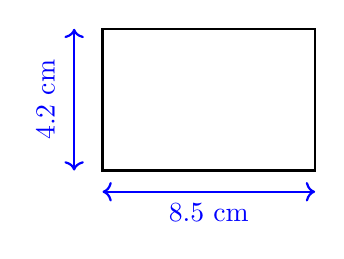
\begin{tikzpicture}[scale=0.9]
  % Rectangle for perimeter
  \draw[thick] (0,0) rectangle (3,2);
  \draw[blue, thick, <->] (0,-0.3) -- (3,-0.3);
  \node[blue] at (1.5,-0.6) {$8.5$ cm};
  \draw[blue, thick, <->] (-0.4,0) -- (-0.4,2);
  \node[blue, rotate=90] at (-0.8,1) {$4.2$ cm};
  
\end{tikzpicture}
\end{center}

\column{0.7\textwidth}
\small
\begin{enumerate}
    \begin{multicols}{2}
        \item $13 + 9 =$ \ashowq{$22$}
        \item $5.8 - 1.9 =$ \ashowq{$3.9$}
    \end{multicols}
    \begin{multicols}{2}
        \item $6 \times 8 =$ \ashowq{$48$}
        \item $4 \times 3.5$ \ashowq{$14$}
    \end{multicols}
  \item Round $3.14159$ to 2 decimal places. \ashow{$3.14$}
  \item A pencil is $12.8$ cm long. How many millimetres is this? \ablank{$128$ mm}
\end{enumerate}

\begin{enumerate}
  \setcounter{enumi}{4}
  \item Find the perimeter of the rectangle shown. \ashow{$25.4$ cm}
  \item The perimeter of a square is $26$ cm. What is the length of one side? \ashow{$6.5$ cm}
  \item  The perimeter of an equilateral triangle is $12.9$ cm. 
    Find the length of one side, and then the perimeter of a regular hexagon with the same side length. \ashow{$4.3$ cm; hexagon: $25.8$ cm}
\end{enumerate}

\end{columns}
\end{frame}

%------------------------------------------------
% SLIDE 2: Arithmetic + Radius, Diameter, Chord
%------------------------------------------------
\begin{frame}{Starter}

\begin{columns}

\column{0.3\textwidth}
\begin{center}
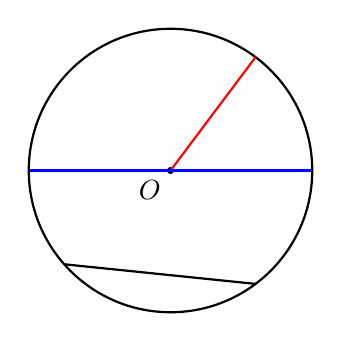
\begin{tikzpicture}[scale=0.9]
  % Circle
  \draw[thick] (0,0) circle (2cm);
  
  % Center
  \fill (0,0) circle (0.05);
  \node[below left] at (0,0) {$O$};
  
  % Radius
  \draw[red, thick] (0,0) -- (1.2,1.6);
  
  % Diameter
  \draw[blue, thick] (-2,0) -- (2,0);
  
  % Chord (not through center)
  \draw[thick] (-1.5,-1.323) -- (1.2,-1.6);

  
\end{tikzpicture}
\end{center}

\column{0.7\textwidth}
\small
\begin{enumerate}
\begin{multicols}{2}
  \item $24 \div 6$ \ashow{$=4$}
  \item $72 \div 8$ \ashow{$=9$}
  \end{multicols}
  \begin{multicols}{2}
  \item Double $15.5$ \ashow{$=31$}
  \item Halve $31.4$ \ashow{$=15.7$}
  \end{multicols}
  \item How many centimetres in $1.2$ metres? \ashow{$120$ cm}
  \item True or false? $2.5 \times 4 = 10$ \ashow{True}
\end{enumerate}

\begin{enumerate}
  \setcounter{enumi}{4}
  \item On the diagram, which line is the \textbf{diameter}? 
    How is it different from a chord? \ashow{Blue line; a diameter passes through the centre.}
  \item If the radius of a circle is $7$ cm, what is its diameter? \ashow{$14$ cm}
  \item The diameter of a circle is $18$ mm. Find its radius. \ablank{$9$ mm}
  \item A chord of length $8$ cm is drawn inside a circle of radius $5$ cm.
    Is the chord a diameter? Explain. \ashow{No; a diameter would be $10$ cm.}
\end{enumerate}

\end{columns}
\end{frame}

%------------------------------------------------
% SLIDE 3: Arithmetic + Segments, Sectors, Arcs, Tangents
%------------------------------------------------
\begin{frame}{Starter}


\begin{columns}

\column{0.35\textwidth}

\begin{center}
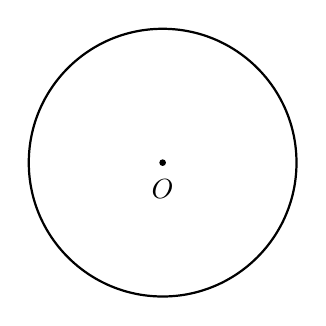
\begin{tikzpicture}[scale=0.85]
  % Circle
  \draw[thick] (0,0) circle (2cm);
  \fill (0,0) circle (0.05);
  \node[below] at (0,-0.1) {$O$};

\end{tikzpicture}

\vspace{3em}

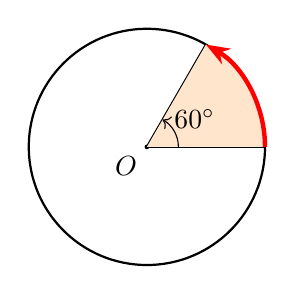
\begin{tikzpicture}[scale=1]
  % Circle
  \draw[thick] (0,0) circle (1.5cm);
  
  % Centre
  \fill (0,0) circle (0.03);
  \node[below left] at (0,0) {$O$};
  
  % Radii that bound the 60° sector
  \draw[thick] (0,0) -- (0:1.5);          % right horizontal radius
  \draw[thick] (0,0) -- (60:1.5);         % radius at 60°
  

  
  % Optional: shade the sector lightly
  \fill[orange!20] (0,0) -- (0:1.5) arc (0:60:1.5) -- cycle;

    % Highlight the arc (thick, coloured, with arrow)
  \draw[red, ultra thick, -{Stealth[length=3mm]}] 
    (0:1.5) arc (0:60:1.5);
  
  % Angle arc and label
  \draw[->] (0.4,0) arc (0:60:0.4);
  \node at (30:0.7) {$60^\circ$};
  
\end{tikzpicture}

\end{center}


\column{0.65\textwidth}
\small
\begin{enumerate}
\begin{multicols}{2}
  \item $3.2 \times 5$ \ashow{$=16$}
  \item $1.8 \times 4$ \ashow{$=7.2$}
  \end{multicols}
  \begin{multicols}{2}
    \item  $45 \div 10$ \ashow{$=4.5$}
    \item $90 \div 100$ \ashow{$=0.9$}
  \end{multicols}
  \item What is $\frac{1}{4}$ of $360^\circ$? \ashow{$90^\circ$}
\end{enumerate}

\begin{enumerate}
  \setcounter{enumi}{5}
  \item Copy the diagram, and draw with labels:
    \begin{multicols}{2}
    \begin{itemize}
      \item A sector
      \item An arc
      \item A tangent
      \item A segment
    \end{itemize}
    \end{multicols}
    \ashow{Sector: shaded slice; Arc: curved boundary; Tangent: line touching the circle once; Segment: region between a chord and an arc.}
  \item If the radius is $6$ cm, what is the whole circumference? (Use $\pi \approx 3.14$) \ashow{$37.68$ cm}
  \item For the sector shown, what fraction of the circumference is the arc length? Calculate the arc length if the whole circle has a circumference of 24cm. \ashow{$\frac{1}{6}$; $4$ cm}

\end{enumerate}

\end{columns}
\end{frame}

%------------------------------------------------
% SLIDE 4: Arithmetic + Labelling, Pi, Diameter
%------------------------------------------------
\begin{frame}{Starter}

\vspace{-2em}

\begin{columns}

\column{0.3\textwidth}
\begin{center}
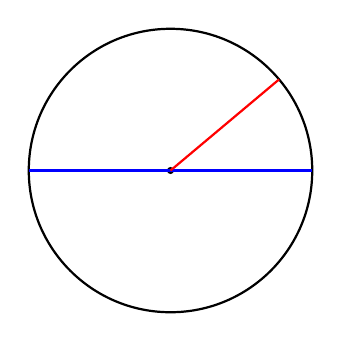
\begin{tikzpicture}[scale=0.9]
  % Circle with labels
  \draw[thick] (0,0) circle (2cm);
  \fill (0,0) circle (0.05);
  
  \draw[blue, thick] (-2,0) -- (2,0);
  
  \draw[red, thick] (0,0) -- (40:2);
  
\end{tikzpicture}

\end{center}

\column{0.7\textwidth}
\small
\begin{enumerate}
\begin{multicols}{2}
  \item $12 \times 3 $ \ashow{$=36$}
  \item $4 \times 3.14$ \ashow{$=12.56$}
\end{multicols}
\begin{multicols}{2}
  \item $6.28 \div 2 $ \ashow{$=3.14$} 
  \item $ 9.42 \div 3$ \ashow{$=3.14$}
  \end{multicols}
  \item Round $3.14159265$ to 3 decimal places. \ashow{$3.142$}
  \begin{multicols}{2}
  \item Double $3.14$ \ashow{$=6.28$}
  \item halve $12.56$ \ashow{$=6.28$}
  \end{multicols}
\end{enumerate}
\vspace{-0.5em}
\begin{enumerate}
  \setcounter{enumi}{7}
  \item Copy and label on the diagram: 
    centre, radius, diameter, circumference. \ashow{centre: $O$; radius: red line; diameter: blue line; circumference: the circle itself}
    \item Draw a chord on the diagram shorter than the radius \ashow{Many possible answers, e.g.\ a chord close to the circumference}
    \item Draw a chord on the diagram longer than the radius \ashow{Many possible answers, e.g.\ a chord passing near the centre but not through it}
  
  \item If the diameter is $8$ cm, what is:
    \begin{itemize}
      \item the radius? \ashow{$4$ cm}
      \item the circumference? ($\pi \approx 3.14$) \ashow{$25.12$ cm}
    \end{itemize}
 
\end{enumerate}

\end{columns}
\end{frame}

\end{document}